\documentclass[a4paper]{article}
\usepackage[bottom=10em]{geometry}

\usepackage[T1]{fontenc}	
\usepackage{amsmath}
\usepackage{amssymb}
\usepackage{graphicx}
\usepackage{fancyhdr}
\usepackage{array}
\usepackage{float}

\pagestyle{fancy}
\lhead{Computer Excercise 1}
\rhead{Kristoffer Nordström, Noah Hansson}

\title{Computer Exercise 1 - NEKN83}
\author{Kristoffer Nordström, Noah Hansson}
\date{\today}

\setlength{\parskip}{0.7em}
\setlength{\parindent}{0pt}
\setlength{\floatsep}{6pt plus 1.0pt minus 2.0pt}
\setlength{\textfloatsep}{10pt plus 1.0pt minus 2.0pt}

\begin{document}

\maketitle

\section{Introduction}
The purpose of this exercise is to implement and evaluate different methods of estimating Value-at-Risk\footnote{Henceforth referred to as VaR} for a given asset. The data used in the exercise consists of price observations for a US-stock market portfolio observed between 2006 - 2008. Value at risk is estimated and evaluated for 2008. Different methods of estimating VaR will then be compared based on how often the losses exceed the VaR estimate.

\section{Method}
In this exercise three different methods of estimating VaR will be used. On top of that, the volatility of the observed losses will be estimated in two different ways. This results in 6 different VaR estimates. To test the reliability of the models the number of violations will be compared to the Kupiec test, giving a 95\% confidence interval of expected violations.
   
The VaR is estimated by using the 99\% percentile of the observed losses. For the regular estimate this is done using Microsoft Excel's percentile\footnote{PERCENTILE.INC()} function. Furthermore, the VaR is also estimated by assuming that the observed losses follows a normal distribution and a T-distribution and then finding the corresponding 99\% percentile.

The first way of modeling volatility will be based on an average standard deviation of historical measurements, by using a 500 days moving average of the volatility of measured losses. The second way of measuring will be based on an EWMA conditional volatility approximation of the GARCH-model to give a one-step prediction of volatility.



\section{Empirical Results}
The exercise is solved in the provided Excel sheet, and the plots are made in python. 

\begin{figure}[H]
    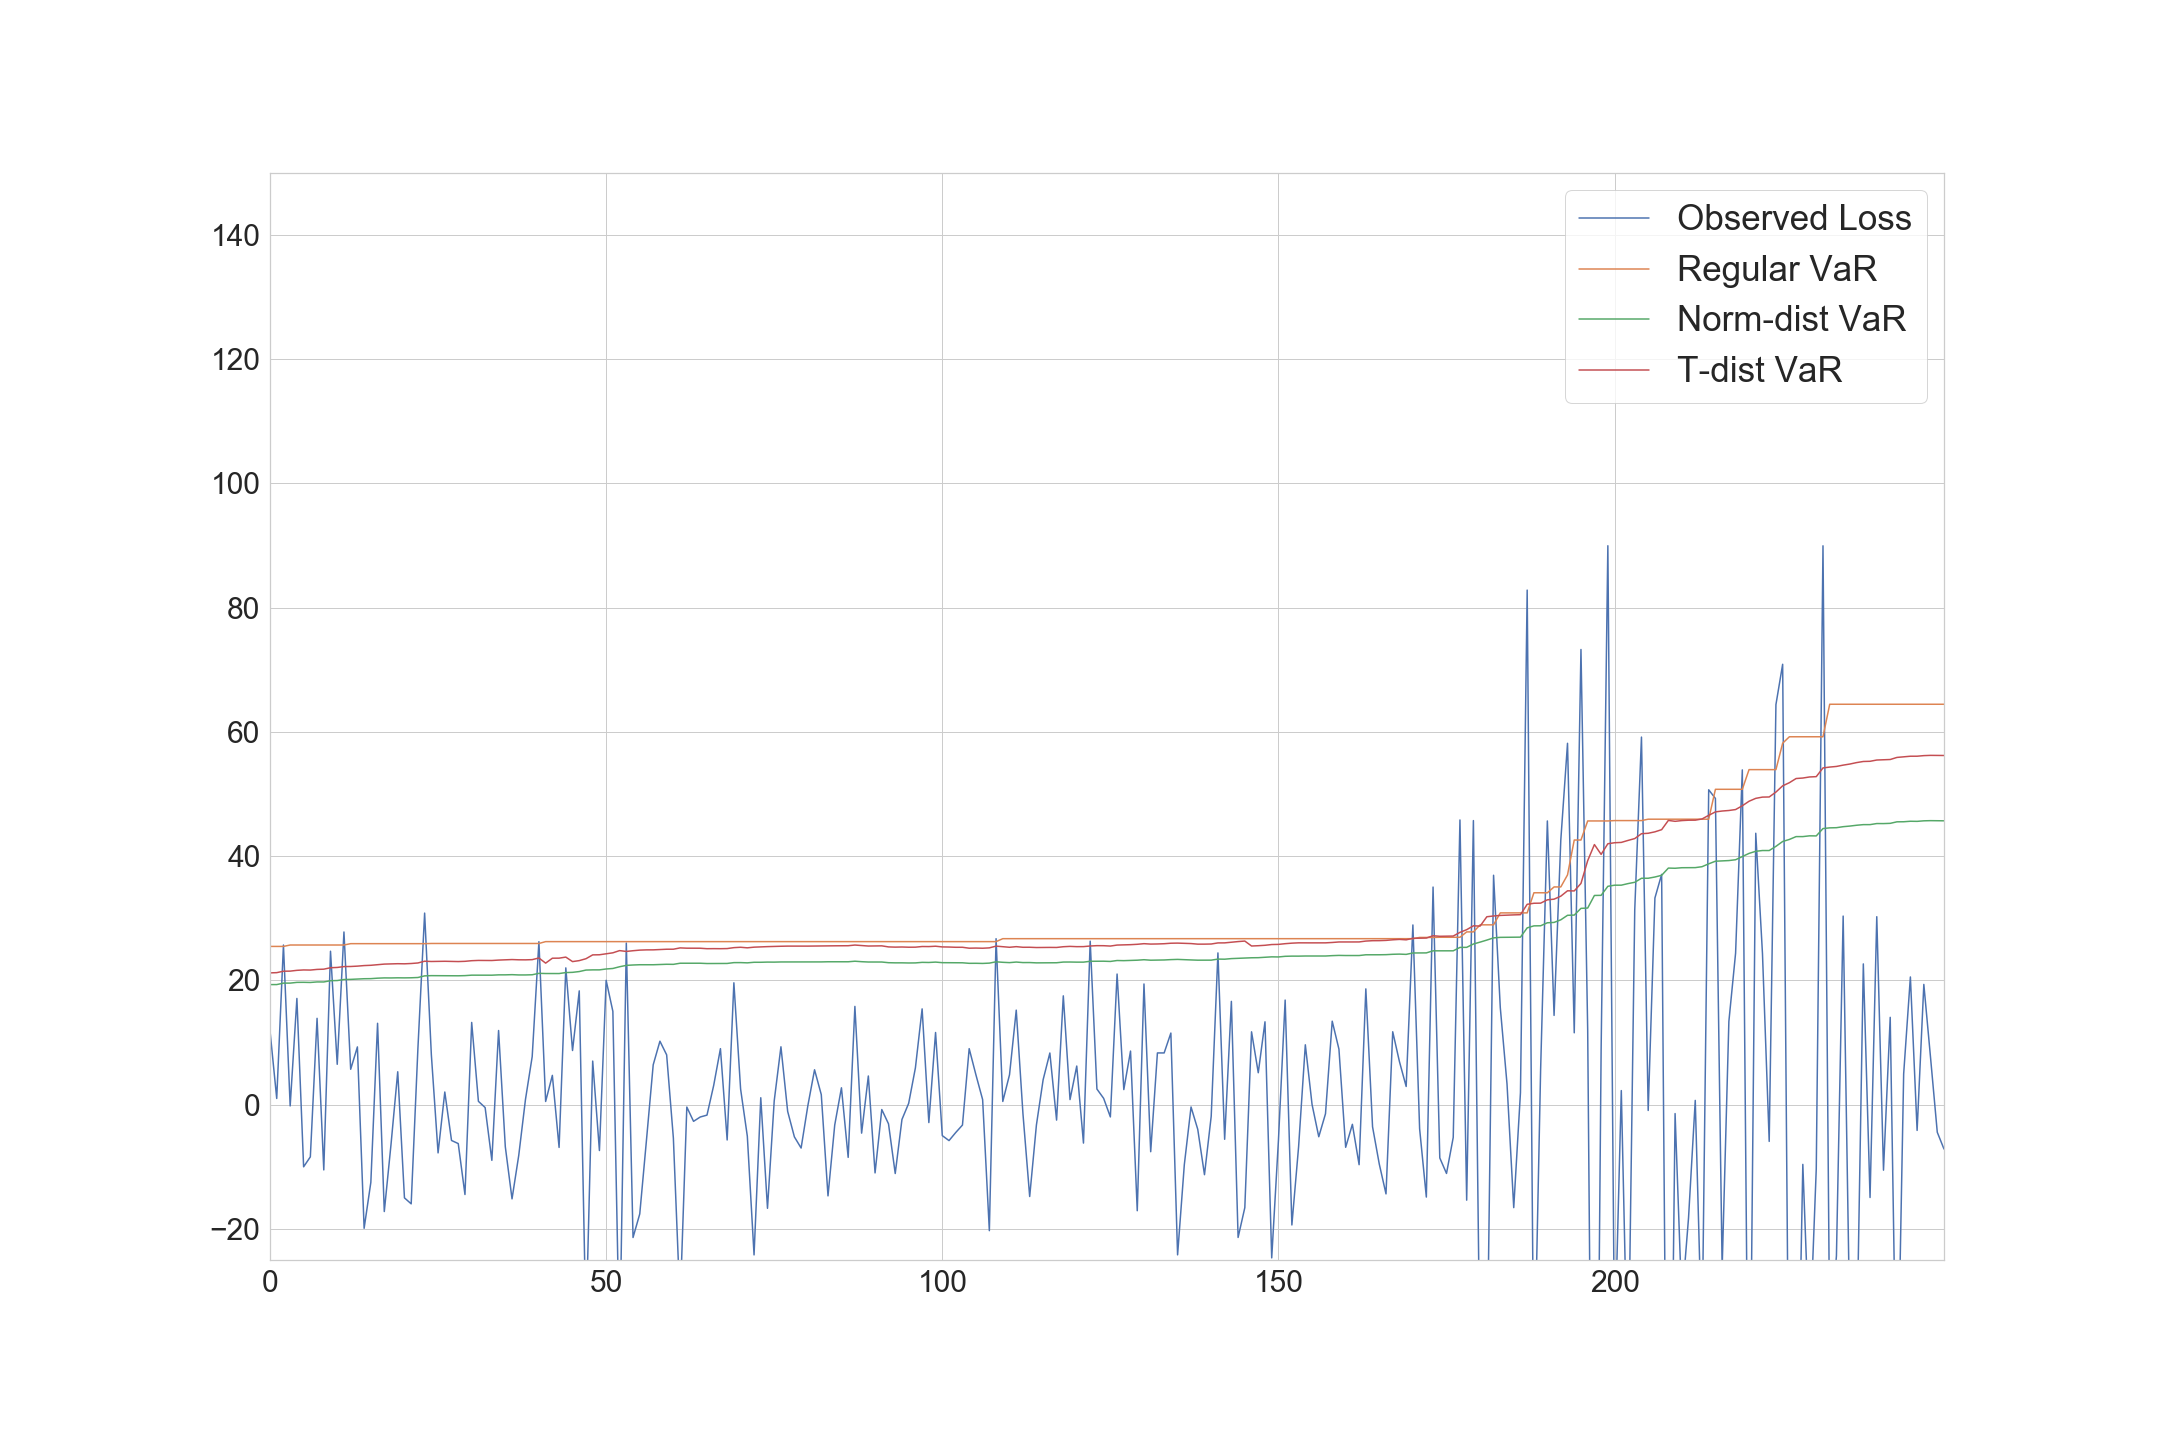
\includegraphics[width=\textwidth]{VaR1.png}
    \caption{Observed loss compared to $VaR_{99\%}$ estimates based on historical volatility}
    \label{var1}
\end{figure}

\begin{figure}[H]
    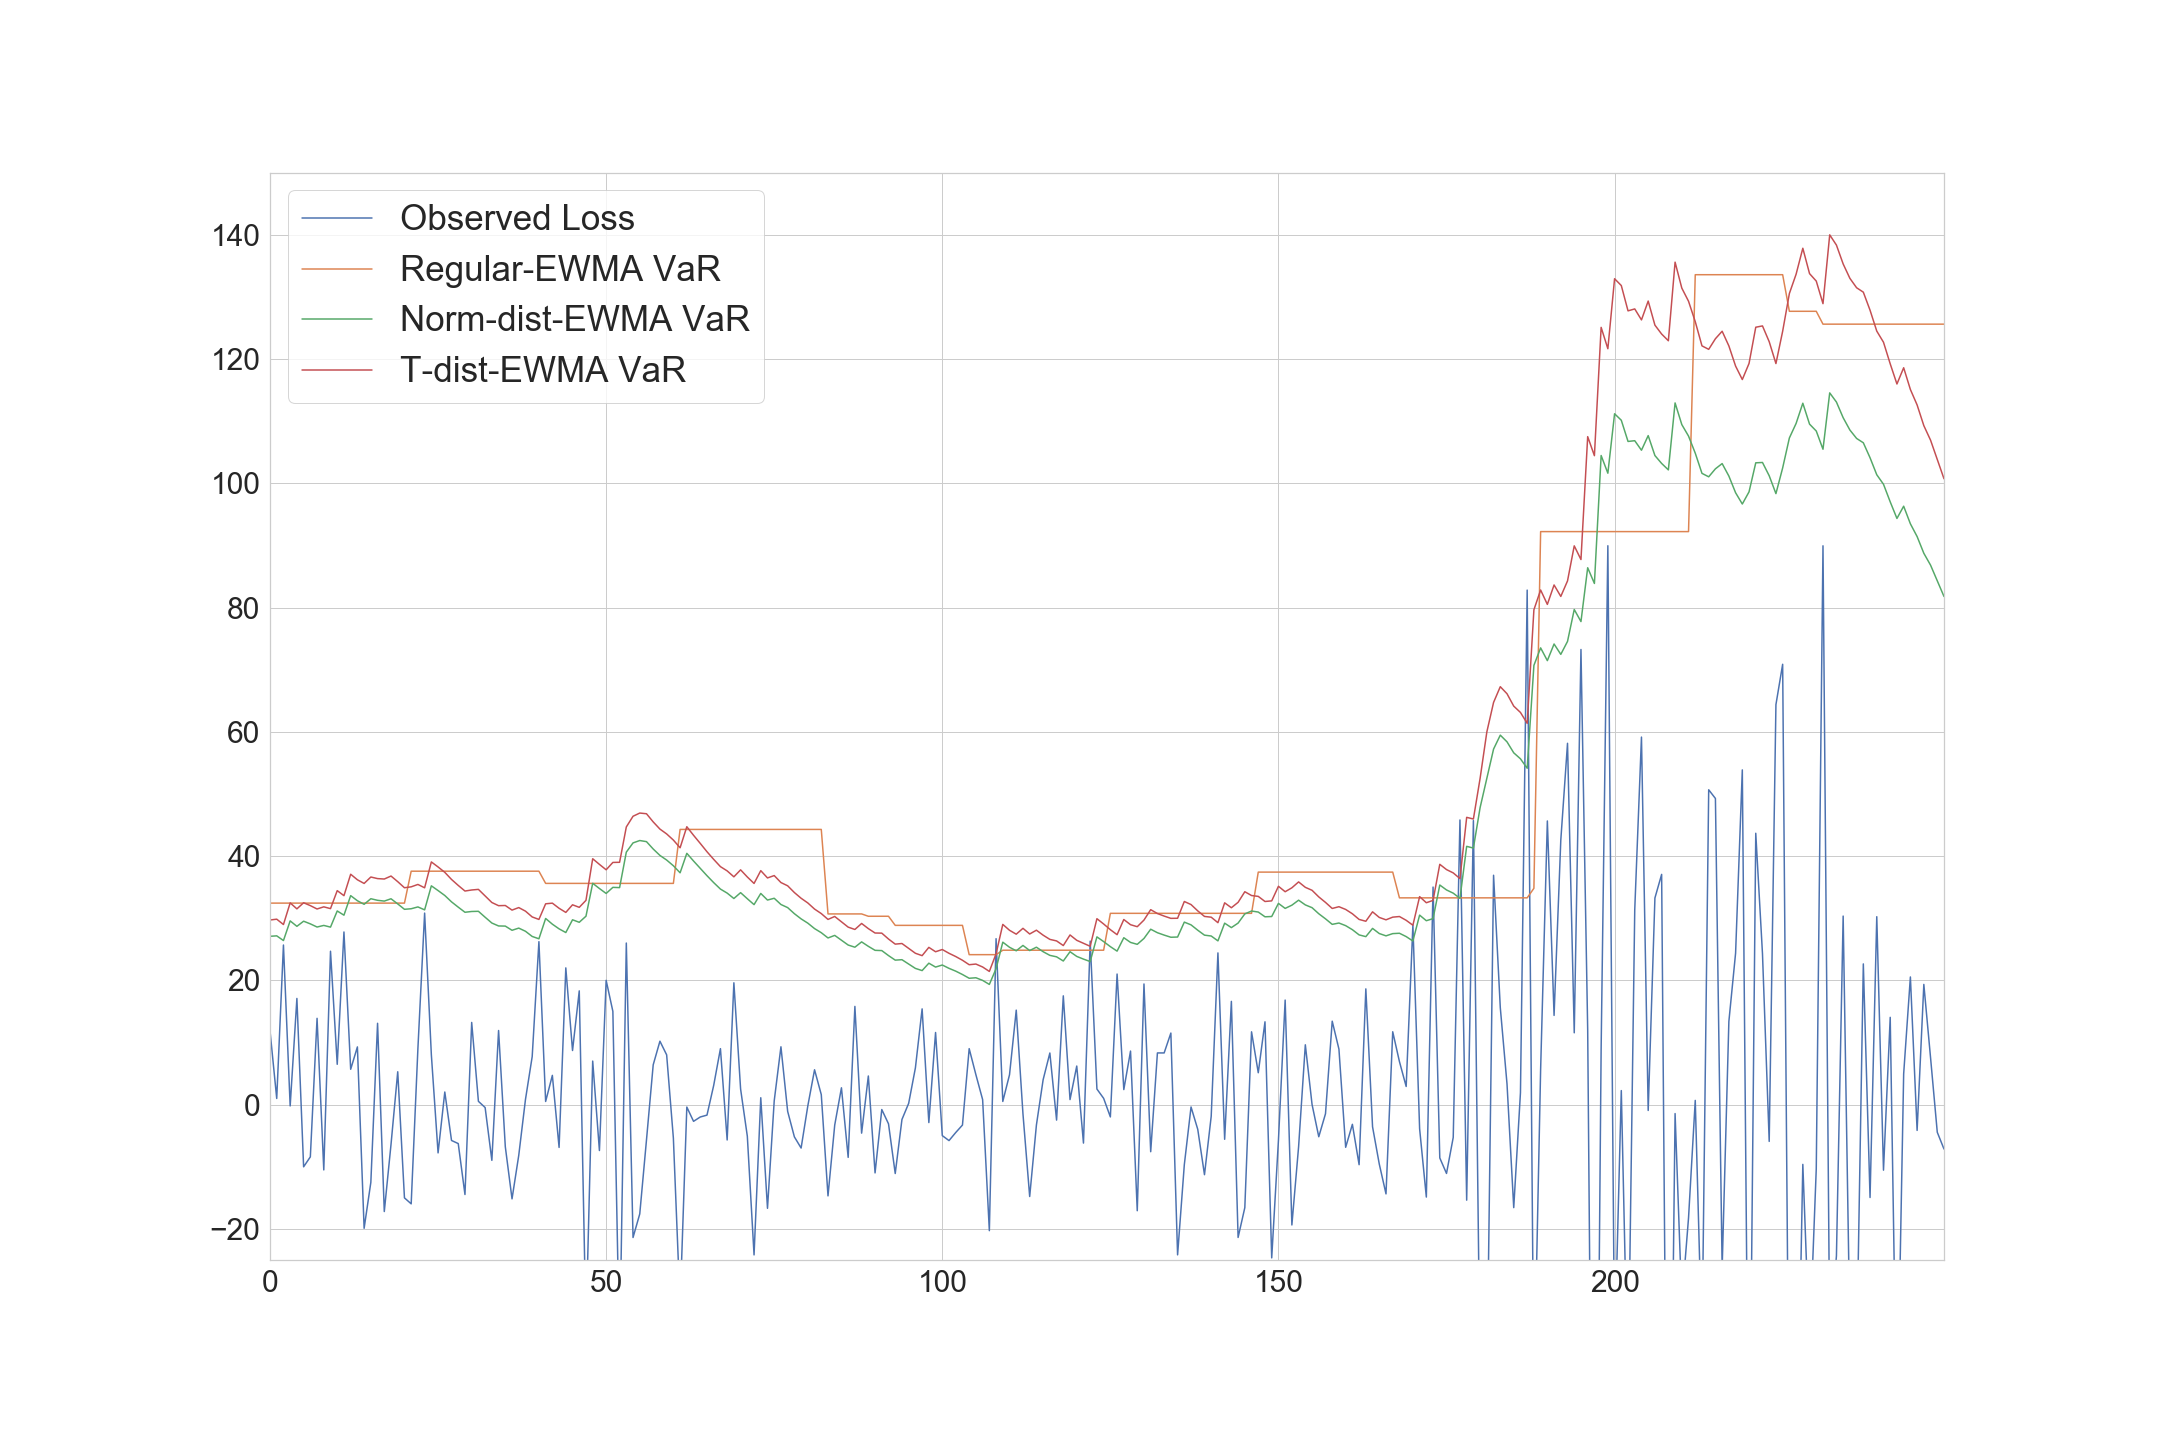
\includegraphics[width=\textwidth]{VaR2.png}
    \caption{Observed loss compared to $VaR_{99\%}$ estimates based on EWMA volatility predictions}
    \label{var2}
\end{figure}

\begin{table}[H]
	\centering
    \caption{95\% Confidence Interval of $VaR_{99\%}$ violations for 250 data points given by the Kupiec test}
    \vspace{0.2cm}
    \begin{tabular}{|c|c|}
        \hline
        Lower Bound & 0  \\ \hline
        Upper Bound & 6  \\\hline
	\end{tabular}
\end{table}

\begin{table}[H]
	\centering
    \caption{Number Of VaR Violations}
    \label{violations}
    \vspace{0.2cm}
    \begin{tabular}{|m{1.8cm}|*6{m{1.2cm}|}}
        \hline
        Volatility model & \multicolumn{3}{c|}{Moving Average} & \multicolumn{3}{c|}{EWMA} \\ 
        \hline
        Loss distribution & Excel & Normal dist & T-dist & Excel & Normal dist & T-Dist\\
        \hline
		Number Of Violations & 22 & 30 & 26 & 7 & 7 & 6 \\\hline
	\end{tabular}
\end{table}


\section{Conclusion}
As seen in table \ref{violations}, using an EWMA volatility predictor gives us a better VaR-estimate. In fact, the only VaR estimate that manages to pass the Kupiec test is the EWMA T-distribution estimate. However, both methods have their pros and cons. Comparing figure \ref{var1} and figure \ref{var2} shows that the EWMA methods better manage to follow the market when volatility spikes, but also results in a higher variance in estimates. This often gives a higher VaR-estimate than necessary when the volatility changes slowly. When this is the case the historical volatility estimates give a lower VaR without causing too many violations.

We can conclude that the choice of volatility model matters a lot more than the underlying assumption of distribution of the loss function. As such, the first step towards making a more reliable estimator would be to find a better predictor of volatility.

\end{document}
